%課題研究レジュメテンプレート ver. 1.1

\documentclass[uplatex]{jsarticle}
\usepackage[top=20mm,bottom=20mm,left=20mm,right=20mm]{geometry}
\usepackage[T1]{fontenc}
\usepackage{txfonts}
\usepackage{wrapfig}
\usepackage[expert,deluxe]{otf}
\usepackage[dvipdfmx,hiresbb]{graphicx}
\usepackage[dvipdfmx]{hyperref}
\usepackage{pxjahyper}
\usepackage{here}



\makeatletter
  \renewcommand{\section}{%
    \if@slide\clearpage\fi
    \@startsection{section}{1}{\z@}%
    {\Cvs \@plus.5\Cdp \@minus.2\Cdp}% 前アキ
    {.5\Cvs \@plus.3\Cdp}% 後アキ
    %{\normalfont\Large\headfont\raggedright}}
    {\normalfont\raggedright}}

  \renewcommand{\subsection}{\@startsection{subsection}{2}{\z@}%
    {\Cvs \@plus.5\Cdp \@minus.2\Cdp}% 前アキ
    {.5\Cvs \@plus.3\Cdp}% 後アキ
    %{\normalfont\large\headfont}}
    {\normalfont}}

  \renewcommand{\subsubsection}{\@startsection{subsubsection}{3}{\z@}%
    {\Cvs \@plus.5\Cdp \@minus.2\Cdp}%
    {\z@}%
    %{\normalfont\normalsize\headfont}}
    {\normalfont}}
\makeatother

\makeatletter
\newcommand{\figcaption}[1]{\def\@captype{figure}\caption{#1}}
\newcommand{\tblcaption}[1]{\def\@captype{table}\caption{#1}}
\makeatother

%ここから上を編集する必要はない.





\title{\vspace{-14mm}GitHubのソフトウェア開発における貢献度分析}
\author{PMコース 矢吹研究室 1342100 春川 直幸}
\date{}%日付を入れる必要はない.
\pagestyle{empty}%ページ番号は振らない.
\begin{document}
\maketitle





\section{研究の背景}

ソフトウェア開発では,複数のメンバが同時に開発を行うため,ファイルの最新バージョンが分からなくなる,同一ファイルに対する変更が競合する等の問題が発生する.このような問題を解決するため,バージョン管理システムを用いる\cite{ikeda2014}.バージョン管理システムとは,変更履歴を管理するシステムのことである.具体的にはソフトウェアのソースコードを書き足したり,変更したりする過程を記録していき,特定の段階まで戻ったり,誤って消してしまったファイルを復活させたりなど,バージョン管理システムはソフトウェア開発の現場において無くてはならない機能である\cite{otuka2014}.

バージョン管理システムを提供するサービスに,GitHubがある.
GitHubにはgit logコマンドというものがある.git logコマンドとは,リポジトリのコミットされたログを確認できるコマンドである.誰がいつコミットやマージをしてどのような差分を発生したのか確認できる\cite{otuka2014}.
このgit logコマンドを解析することにより,コミットによる開発者の貢献度を求め,GitHubでのソフトウェア開発でもパレートの法則が成り立つのか調査する.

\section{研究の目的}

GitHubを用いたソフトウェア開発プロジェクトにおいて,コミット数によるプロジェクトへの貢献度を可視化し,結果を分析する.

\section{プロジェクトマネジメントとの関連}

コミットによるプロジェクトの貢献度を分析しパレート図を作成することにより,GitHub を用いたソフトウェア開発プロジェクトで,プロジェクトの管理上の優先度を明示させる.
これはプロジェクトマネジメントの知識エリアにおいて,品質マネジメントに該当する.


\section{研究の方法}




本研究は2段階に分かれる.
\begin{enumerate}
\item シェル(Shell)を使用し,GitHub上のプロジェクトから,開発者数とコミット回数を調査する.
\item 調査したデータの分析をする.
\end{enumerate}


調査したデータの分析は,デシル分析で行う.
デシル分析とは,購買履歴データをもとに全顧客の購入金額を高い順に10等分して、各ランク(デシル1~10)の購入比率や売上高構成比を算出する主にマーケティングで使用する分析方法のことである\cite{decyl01}.
今回はデシル分析でコミット数の多い順に10等分して,各ランク(デシル1~デシル10)のコミット比率を算出し,コミット貢献度を明らかにする.




\section{現在の進捗状況}



GitHub上の10個のプロジェクトから,プロジェクトの開発者数、コミット数を調査し,デシル分析を行った.

開発者人数は最少1人,最大3503人だった.コミット数は最小1,最大54421だった.

10件のプロジェクトをデシル分析し平均を算出した.結果は,表1である.表1をグラフ化したものが図2になる.分析結果から,デシル1の構成比が88%になっており,約9割の成果は1割の開発者によって生み出されていることがわかった.

こうなった要因として調査したすべてのプロジェクトでオーナーのコミット数が一位だったことが関係していると考える.コミット数が一位だった開発者の構成比の平均を求めた結果,42.4%だった.

このことから,GitHubにおけるソフトウェア開発では,パレートの法則とは若干違う結果になっていると言えるであろう.



\begin{table}[h] 
\centering
 \tblcaption{デシル分析 表} \label{デシル分析}
\begin{tabular}{|c|c|c|c|}
\hline
セグメント & 計コミット数 & 構成比 & 累積構成比 \\
\hline
  デシル1 & 7833 & 88.0% & 88.0% \\
  デシル2 & 321 & 3.6% & 91.6% \\
  デシル3 & 171 & 1.9% & 93.5% \\
  デシル4 & 124 & 1.4% & 94.9% \\
  デシル5 & 93 & 1.0% & 95.9% \\
  デシル6 & 73 & 0.8% & 96.8% \\
  デシル7 & 73 & 0.8% & 97.6% \\
  デシル8 & 73 & 0.8% & 98.4% \\
  デシル9 & 73 & 0.8% & 99.2% \\
  デシル10 & 71 & 0.8% & 100% \\
\hline
\end{tabular}\end{table}

\begin{figure}[H] 
\centering
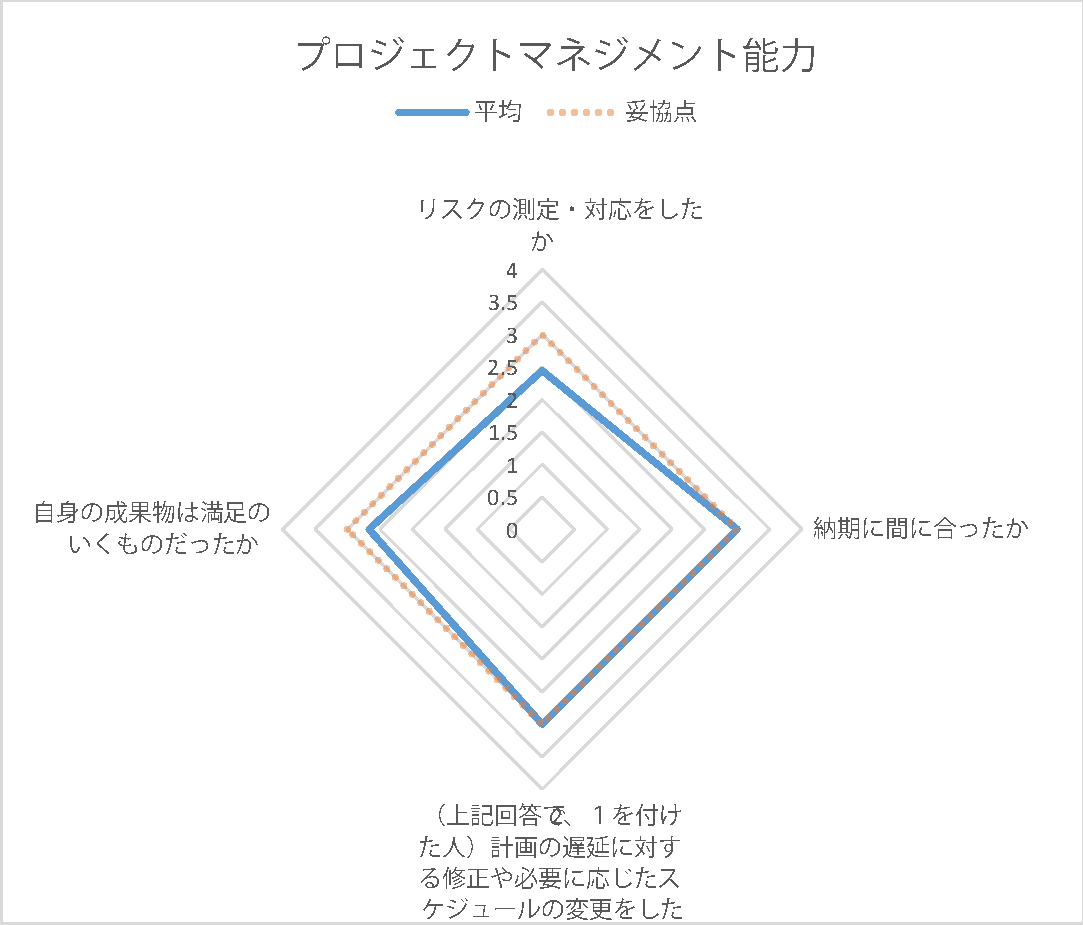
\includegraphics[width=13cm]{g1.pdf}
\caption{デシル分析 グラフ}\label{デシル分析}
\end{figure}	

\section{今後の計画}

以下のように研究を進める計画である.

\begin{enumerate}
\item データを自動で集められるように環境を整える. 
\item 調査対象となるプロジェクトの数を増やしたり,他の分析手法も用いて分析を行う.
\item 論文の執筆を行う.

\end{enumerate}

\bibliographystyle{junsrt}
\bibliography{biblio}%「biblio.bib」というファイルが必要.

\end{document}
